
%
% realization - architecture + implementation
%

\section{Architecture \& Implementation}
\label{chapter:architecture-implementation}

Geocluster is a Drupal 7 module that implements the Geohash-based clustering algorithm. 
 
An iterative approach was taken in order to explore ways to fulfill the various integration and extensibility requirements formulated in chapter \ref{chapter:objective-performance} and analyzed in chapter \label{chapter:analysis-drupal}. Based on the Drupal mapping stack explained in chapter \ref{chapter:drupal-mapping}, a high-level architecture for implementing the Geohash-based clustering algorithm was designed.

\subsection{Principles}

Geocluster has been implemented following a number of principles:

\begin{itemize}

\item Leverage existing APIs and \textit{hooks} when possible
\item Program object-oriented code where it makes sense
\item Implement changes to existing modules as \textit{patches} if necessary

\end{itemize}

While using APIs and object-oriented programming are familiar concepts, \textit{hooks} are a Drupal-specific concept. They basically allow modules to interact with each other in a procedural way in which many parts of the Drupal system are built.

\begin{quote}
Drupal's module system is based on the concept of "hooks". A hook is a PHP function that is named foo\_bar(), where "foo" is the name of the module (whose filename is thus foo.module) and "bar" is the name of the hook. Each hook has a defined set of parameters and a specified result type.

To extend Drupal, a module need simply implement a hook. When Drupal wishes to allow intervention from modules, it determines which modules implement a hook and calls that hook in all enabled modules that implement it.\footnote{\url{http://api.drupal.org/api/drupal/includes!module.inc/group/hooks/7}}
\end{quote}

The term \textit{patch} describes a way to submit code changes used within the Drupal and other open source communities:

\begin{quote}
Patches are pieces of code that solve an existing issue. In fact, patches describe the changes between a before and after state of either a module or core. By applying the patch the issue should no longer exist.

Patches are used to maintain control-ability over the entire Drupal project. While Drupal is distributed via the git version control system, patches are additional pieces of code that focus on a single change request and therefore are easily tested, reviewed and documented.\footnote{\url{http://drupal.org/patch}}
\end{quote}



\subsection{Architecture overview}

The parts involved in the Geocluster system are

\begin{itemize}

\item Integration of the Geohash-based hierarchical spatial index with Geofield

\item Server-side clustering implementation
  \begin{itemize}
   \item Configuration of the clustering process
   \item Integration of the clustering process with Views
   \item Implementation of the clustering algorithm
  \end{itemize}

\item Client-side Geocluster Visualization component

\end{itemize}


\begin{figure}[h]
  \begin{center}
    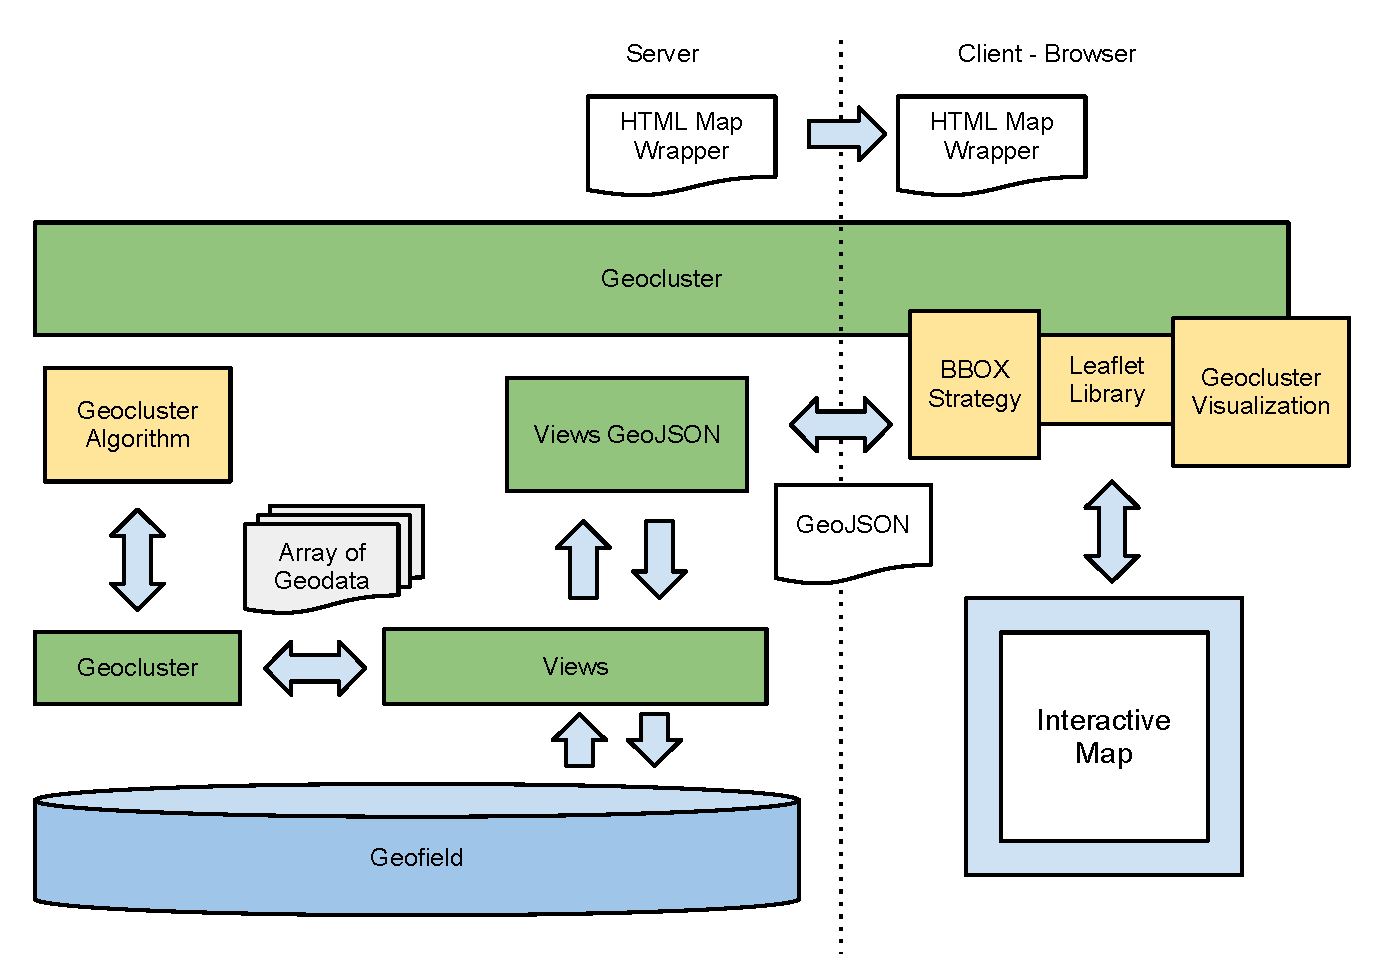
\includegraphics[width=1\textwidth]{figures/geocluster_architecture.pdf}
    \caption{Geocluster architecture overview.}
    \label{fig:geocluster-architecture}
  \end{center}
\end{figure}

Figure \ref{fig:geocluster-architecture} depicts how the Geocluster module integrates with other components of the Drupal mapping stack. The main point of integration for the Geocluster module on the server-side is the Views module. When the Views module performs a spatial query that has been configured for clustering, Geocluster will integrate the clustering algorithm into the Views execution process. The clustering task may interact with the Views module \textit{before} and \textit{after} a query has been executed. Different algorithm implementations may rely on modification of the Views query while others only need to post-process the results of a Views query. After the clustering process has been finished, the server-side execution process continues as usual. The clustered result data is rendered, for example as GeoJSON feed using the Views GeoJSON as indicated in the diagram. On the client-side, a Geocluster Visualization component is used to properly visualize clustered results. The Geocluster module therefore integrates with the Leaflet and Leaflet GeoJSON modules in order extend the Bounding-Box driven communication of clustered results between client and server.


\subsection{Integration of the Geohash-based hierarchical spatial index with Geofield}

The Drupal Field API that Geofield uses has been leveraged to spatially index locations stored by the Geofield module. The field schema for fields of the Geofield type is extended by $geocluster\_field\_schema\_alter$ to add separate columns for the Geohash indices that form the spatial index. The $geocluster\_field\_attach\_presave$ hook implementation takes care of saving the additional index information whenever a Geofield location value is saved to the database.

During the development of the Geocluster module, support for encoding location values into Geohash has been added to the geoPHP library\footnote{\url{https://github.com/phayes/geoPHP/issues/32}}. Subsequently, a patch to make use of geoPHP's Geohash support has been created for the Geofield module and committed\footnote{\url{http://drupal.org/node/1662584}}. 


\subsection{Server-clustering implementation}

The server-side clustering implementation consists of three parts: configuration of the clustering process, integration of the clustering process with Views and implementation of the clustering algorithm.

\begin{figure}[h]
  \begin{center}
    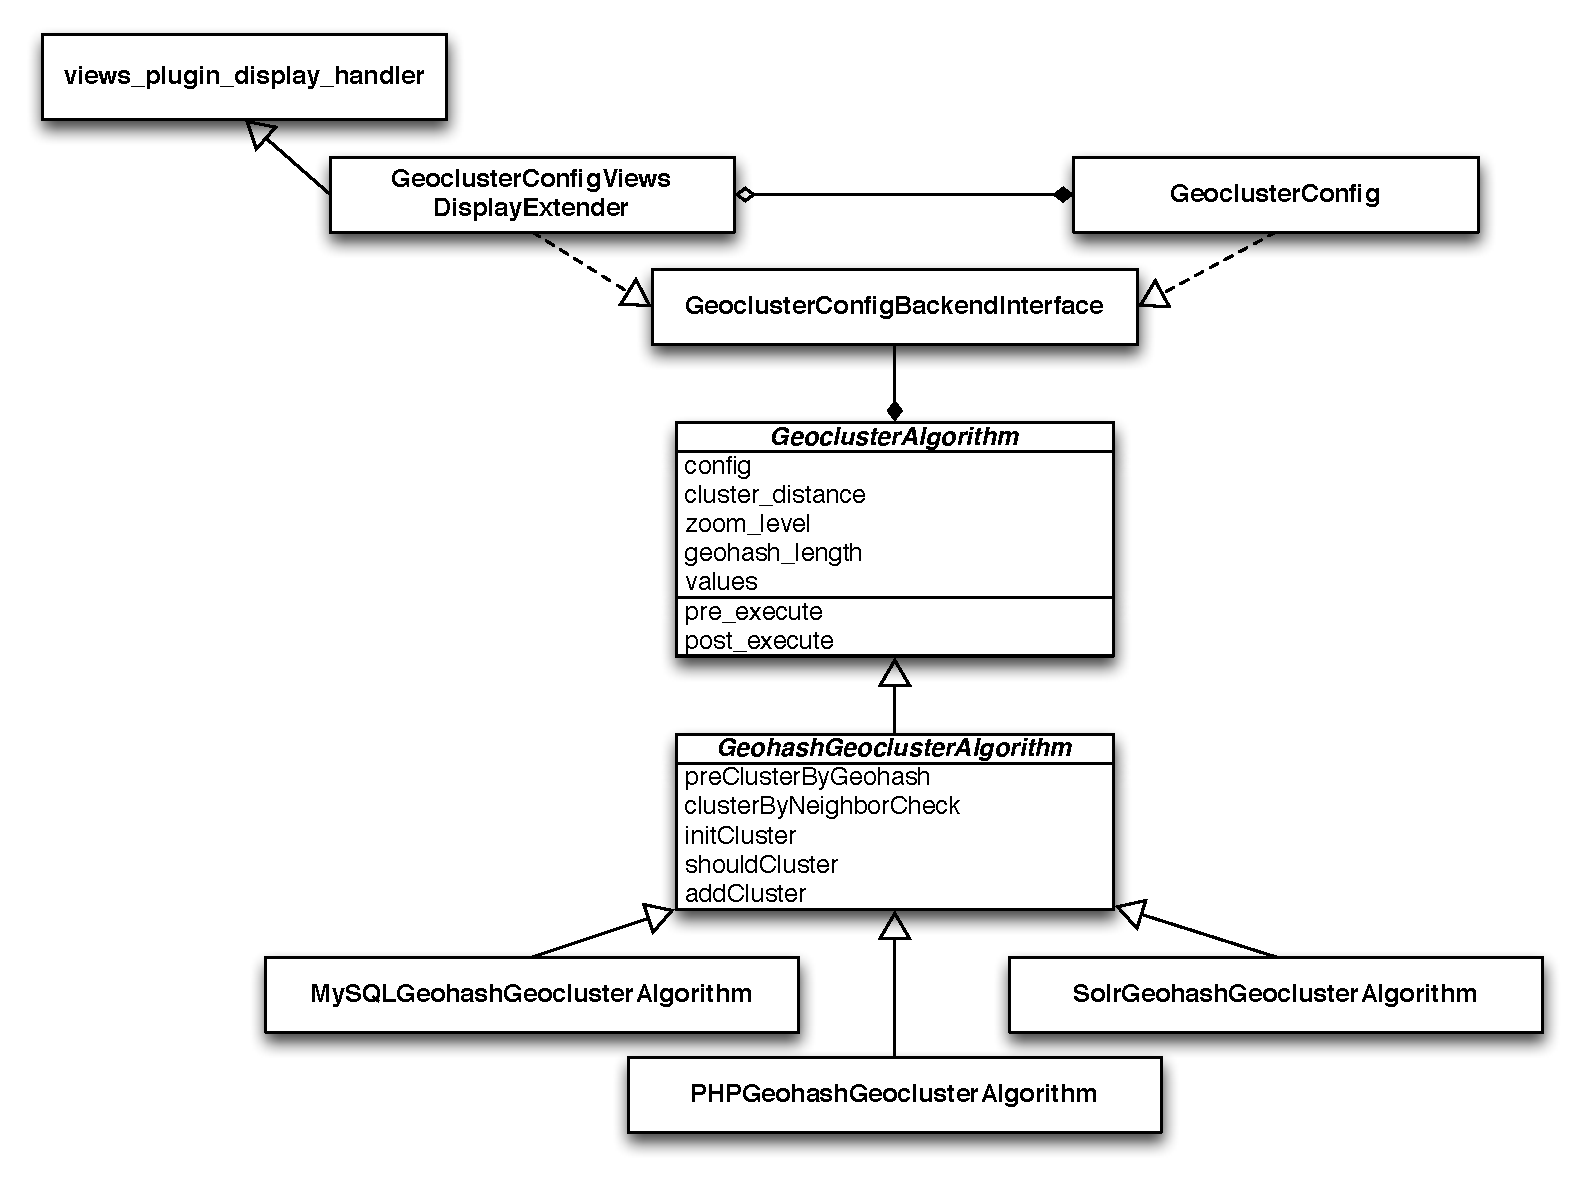
\includegraphics[width=1\textwidth]{figures/geocluster_class_diagram.pdf}
    \caption{Geocluster class diagram.}
    \label{fig:geocluster-class-diagram}
  \end{center}
\end{figure}

Figure \ref{fig:geocluster-class-diagram} illustrates how the \textit{GeoclusterAlgorithm} allows for different variations of the clustering algorithm to be implemented and how the configuration integrates with the Views module. 


\subsection{Configuration of the clustering process}

The Geocluster algorithm depends on three inputs: the data points to cluster, the current zoom level and the minimum cluster distance. The zoom level is passed by the bounding box strategy as a request parameter. In order to configure the rest of the inputs required by the algorithm, a user interface for configuration of the clustering process has been created using the Views plugin system.

When configuring a View, the user may enable Geocluster using a checkbox as illustrated in figure \ref{fig:geocluster-configuration}. If enabled, an additional option set for the clustering process will be displayed.

\begin{itemize}

\item The \textbf{Clustering algorithm} option allows the user to select one of the provided clustering algorithms.

\item The \textbf{Cluster field} option determines the Geofield which should be used as spatial data source for the clustering process. 

\item The \textbf{Cluster distance} option specifies the minimum distance between clusters for the algorithm.

\end{itemize}

\begin{figure}[h]
  \begin{center}
    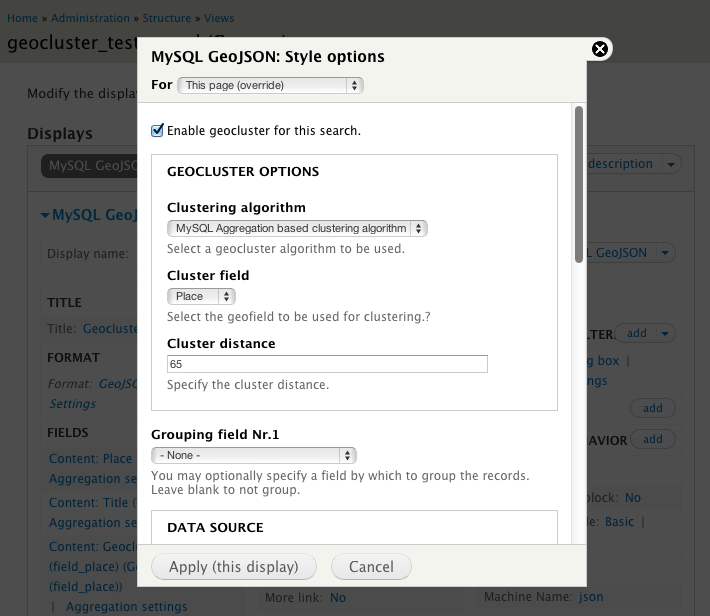
\includegraphics[width=1\textwidth]{figures/geocluster_configuration.png}
    \caption{Geocluster configuration options within the Views administration interface.}
    \label{fig:geocluster-configuration}
  \end{center}
\end{figure}

As indicated by figure \ref{fig:geocluster-class-diagram}, the \textit{GeoclusterConfigViewsDisplayExtender} class integrates the configuration options as a Views plugin. The actual configuration options have been decoupled from the Views-dependent plugin as the \textit{GeoclusterConfig} class. The interface \textit{GeoclusterConfigBackendInterface} abstracts the communication between the configuration classes and the \textit{GeoclusterAlgorithm}. 


\subsection{Implementation of the clustering algorithm}

Three variations of the Geohash-based algorithm have been implemented for Drupal 7. In a first iteration, a \textit{PHP-based} implementation of the clustering algorithm was prototyped to figure out the integration of the algorithm into the Drupal mapping stack. In a second and third iteration, \textit{MySQL-aggregation-based} and \textit{Solr-based} algorithm implementations were added to improve performance and support additional use cases.

The abstract \textit{GeoclusterAlgorithm} class defines the basics of a clustering algorithm. A constructor initializes the clustering task according to phase 1 of the algorithm. The algorithm base class provides access to the configuration options for the algorithm. In addition, it defines $pre\_execute$ and $post\_execute$ as the two main methods that will allow the actual algorithm implementation perform its clustering task.

A second, abstract \textit{GeohashGeoclusterAlgorithm} class encapsulates common infrastructure for the Geohash-based clustering algorithms. An empty stub for creating an initial clustering by using the geohash grid is defined as $preClusterByGeohash$, as well as a default implementation of $clusterByNeighborCheck$ that creates final clusters by checking for overlapping neighbors. Further methods are common helper function defined by the algorithm as $initCluster$, $shouldCluster$ and $addCluster$.

The actual implementations of the geocluster algorithm are realized as plugins using the CTools plugin system\footnote{\url{http://drupal.org/project/ctools}}. This allows other modules to implement their own algorithm plugins which will automatically be exposed within the geocluster configuration options. As an example, the Apache Solr-based geocluster implementation has been implemented within a separate, optional sub-module \textit{Geocluster Solr}. 

\begin{itemize}

\item \textbf{PHPGeohashGeoclusterAlgorithm} is an exemplary, PHP-based implementation of the Geohash-based clustering algorithm. It was primarily created as a first prototype to demonstrate clustering functionality, test the algorithm and work out integration issues with Drupal.

The PHP-based algorithm is completely decoupled from the database, as it only relies on Geofield and performs all clustering logic from phases 2 \& 3 in a the post-execution step of the algorithm. On the other hand, this also makes it the least performant algorithm implementation, because the entire set of results has to be loaded before the clustering process is executed.

\textit{PHPGeohashGeoclusterAlgorithm} uses an adapted version of the \\ \textit{views\_handler\_field\_field::post\_execute()}\footnote{\url{http://api.drupal.org/api/views/modules!field!views\_handler\_field\_field.inc/function/views\_handler\_field\_field\%3A\%3Apost\_execute/7}} method. Its intention is to use\\ \textit{field\_attach\_load}\footnote{\url{http://btmash.com/article/2012-04-13/i-just-want-one-field-using-fieldattachload}} to load just the necessary field information instead of loading items whole entities before the clustering process.


\item \textbf{MySQLGeohashGeoclusterAlgorithm} is a MySQL-aggregation-based implementation of the clustering algorithm. Its intention is to improve performance by shifting the time-critical part from phase 2 of the clustering process into the database. In comparison to the post-execution based PHP algorithm, the database query delivers an already pre-clustered result. The neighbor-check of the algorithm is then performed on the pre-clustered result from the database.

The Geohash-based pre-clustering is realized as a combination of the \textit{GROUP BY} clause with \textit{aggregate} functions. The pre-execution step of the algorithm adds the clustering-specific aggregation settings to the query. The results will be grouped by the column that matches the index level determined by the clustering initialization step. In addition, a the $COUNT$ function is used to calculate cluster sizes and $AVG$ provides an approximation of each cluster's centroid.

\item \textbf{SolrGeohashGeoclusterAlgorithm} is a Search API Solr-based implementation of the clustering algorithm. It improves performance by shifting the time-critical part from phase 2 of the clustering process into the Solr search engine, similarly to the approach of the MySQL-based algorithm. 

Clustering with Solr requires the Geohash-based spatial index to be integrated with the Solr search engine. Also the execution process of a Search API based view differs from the default Views execution process in a number of ways. Finally, the results being processed in a Sarch API View have a different structure from the default result structure of a views result. The resulting complexity of integration of Geocluster with Search API Solr motivated the creation of a separate sub-module \textit{Geocluster Solr} that contains necessary infrastructure and helpers.

\begin{figure}[h]
  \begin{center}
    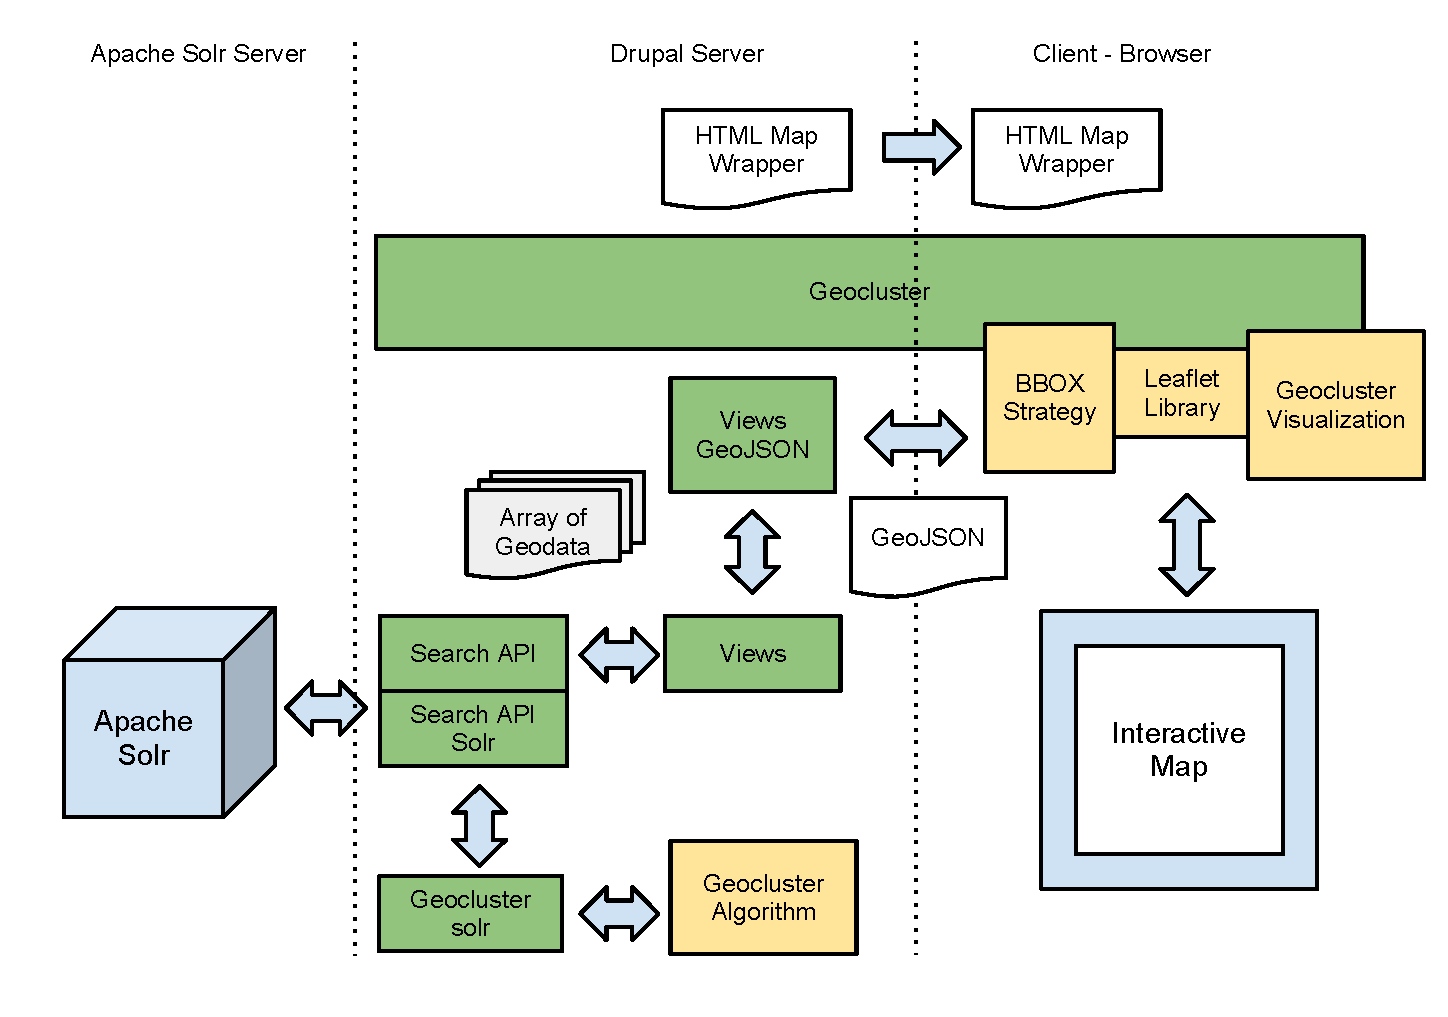
\includegraphics[width=1\textwidth]{figures/geocluster_solr_architecture.pdf}
    \caption{Geocluster Solr architecture overview.}
    \label{fig:geocluster-solr-architecture}
  \end{center}
\end{figure}

Figure \ref{fig:geocluster-solr-architecture} visualizes how Geocluster Solr is integrated into the default architecture of Geocluster, as described in figure \ref{fig:geocluster-architecture}. The original intention was to create a Solr plugin that would perform the entire algorithm within the Solr search engine. A draft for such a plugin has been created on github\footnote{\url{https://github.com/dasjo/SolrGeocluster}}. In order to facilitate the use of Geocluster Solr without the need for installing an custom Solr plugin and for the lack of understanding of the Solr API, a simpler approach was taken. Instead of performing the entire clustering process within Solr, just the first step of creating clusters based on Geohash is realized using a standard Solr query. This still keeps the time critical task within Solr.

A custom search service class $GeoclusterSearchApiSolrService$ has been defined that implements the main clustering logic within a $preQuery$ and a $postQuery$ method. Within the preQuery step, the Geohash-based pre-clustering step is configured by using the \textit{result grouping}\footnote{\url{http://wiki.apache.org/solr/FieldCollapsing}} feature of Apache Solr. The query is configured to return groups of results based on the clustering index level. The postQuery step maps the Solr-based results into a processable structure and delegates to the generic $clusterByNeighborCheck$ method of the clustering algorithm.

\end{itemize}

Two helper classes support the clustering task. $GeoclusterHelper$ provides a set of geospatial PHP functions to in order to calculate the distance between two points on the map in pixels based on the zoom resolution and the haversine formula\footnote{\url{http://en.wikipedia.org/wiki/Haversine_formula}}. Additional helpers support coordinate system conversions for the Spherical Mercator projection, see chapters \ref{chapter:coordinates} and \ref{chapter:projections}. $GeohashHelper$ helps initializing the algorithm by a $lengthFromDistance$ function that determines the appropriate geohash prefix length based on zoom level and minimum distance in pixels.


\subsection{Client-side Geocluster Visualization component}

A simple Geocluster visualization component has been built to support the display of clustered markers on interactive maps based on the output of the server-side clustering implementation. It extends the Bounding Box strategy of the Leaflet GeoJSON module in oder to create numbered markers that visualize the cluster sizes. Clicking on a clustered marker will zoom into the map in order to explore the data on a more granular level. Figure \ref{fig:geocluster-visualiation} demonstrates an example screenshot of the Geocluster visualization.

\begin{figure}[h]
  \begin{center}
    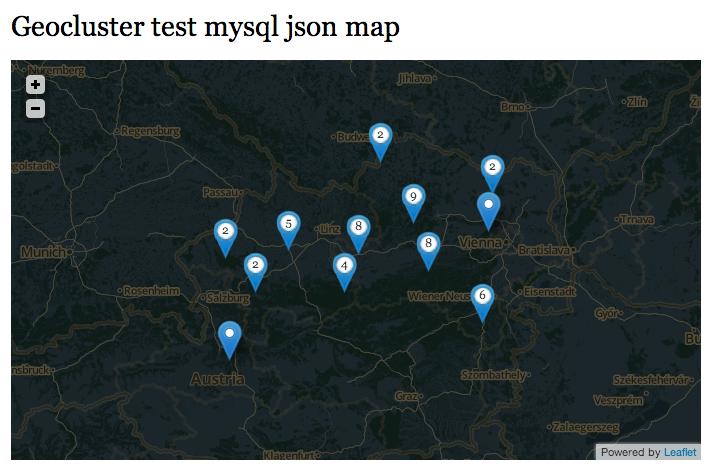
\includegraphics[width=1\textwidth]{figures/geocluster_visualization.png}
    \caption{Geocluster visualization: a Leaflet map containing clustered markers.}
    \label{fig:geocluster-visualiation}
  \end{center}
\end{figure}


The Bounding Box related logic for Leaflet originally has been developed as a part of the Geocluster module. During the development process, this part of Geocluster was generalized and published as the independent Leaflet GeoJSON module\footnote{\url{http://drupal.org/project/leaflet_geojson}}. The visualization component of Geocluster therefore integrates with Leaflet GeoJSON and extends the JavaScript implementation of the Bounding Box strategy to integrate custom markers and cluster interaction. The cluster visualization is based on a code snippet for numbered markers on github\footnote{\url{https://gist.github.com/comp615/2288108}}.